\documentclass[11pt]{article}
\usepackage[final]{acl}
\usepackage{times}
\usepackage{latexsym}
\usepackage[T1]{fontenc}
\usepackage[utf8]{inputenc}
\usepackage{microtype}
% The official template's optional inconsolata package is not required.
\usepackage{graphicx}
\usepackage{amsmath,amssymb}
\usepackage{booktabs}
\usepackage{balance}
\graphicspath{{figures/}}

\title{Activation Survival, Language Association, and Causal Effects\\
under Weight Quantization: A Multilingual SAE Study}
\author{Hemang Joshi \and Eashaan Thakur \and Shardul Joshi \and Nikhita Ravi\\
International Institute of Information Technology, Hyderabad}

\begin{document}
\maketitle

\begin{abstract}
Quantization changes sparse autoencoder (SAE) activations, but an activation change need not imply a loss of language association or causal contribution. We examine these distinctions in Gemma-2-2B using a frozen layer-12 Gemma Scope SAE, 27 FLORES-200 languages, and round-to-nearest weight quantization from INT8 to INT4. Of 8,086 development-selected features, 82.4\% reproduce their original language peak in full precision; among these, 70.8\% retain it at INT4. Removing top-64 language groups increases next-token loss beyond activity-matched controls in all 27 languages, and this dependence persists through INT5. However, the frozen Belebele comprehension test does not establish a corresponding group effect. Individual intervention effects drift at lower precision, but matched alternative directions drift similarly. Graded feature scaling reveals a small INT4 improvement at a 1.1 multiplier, without supporting a simple activation-shrinkage explanation. These results qualify the interpretation of feature survival and do not establish selective-feature destruction as the mechanism of multilingual quantization damage.
\end{abstract}

\section{Introduction}
Weight quantization reduces the numerical precision required to store language-model parameters. Its effects need not be uniform across languages or tasks: multilingual evaluations find disparities that aggregate automatic scores can underestimate \citep{marchisio-etal-2024-quantization}. This motivates examining internal representations alongside model performance. An internal measurement is useful, however, only if its interpretation is explicit. Calling a feature ``lost'' can refer to a change in its activation pattern, preferred language, or effect on predictions. These are different outcomes.

Sparse autoencoders decompose a model activation into a sparse combination of learned directions. Language-associated SAE features have been identified and manipulated in full-precision models \citep{deng-etal-2025-unveiling}. Separately, \citet{duan2026} measure activation correlations before and after weight quantization using a frozen SAE. Neither observation, by itself, establishes that quantization removes language-specific functionality. The representation can change while a contribution remains, or an intervention can change because the downstream model changes.

We initially investigated whether language-selective features were more vulnerable than non-selective controls and whether that difference explained resource-tier disparities. After implementation audits and negative primary contrasts, we expanded the project to test the measurement assumptions directly. This report presents the completed investigation, including hypotheses that were not supported, rather than treating every additional analysis as confirmation of the original question.

We address three questions. \textbf{RQ1:} how do activation preservation and language-association retention compare? \textbf{RQ2:} do selected language groups contribute to prediction and reading comprehension, and how do those contributions change with precision? \textbf{RQ3:} do individual intervention effects and graded group manipulations support an interpretation of feature-specific functional damage?

Our empirical contribution is a controlled case study combining per-language response profiles, native interventions, donor patches, and effect fingerprints across weight precisions. We also document the sensitivity of the initial replication to beginning-of-sequence (BOS) handling. We make no claim that ablation, activation patching, or feature-effect fingerprints are new methods. The main outcome is a set of distinctions and counterexamples to an overly broad interpretation of activation survival, within one model and measurement basis.

\section{Related Work}
\paragraph{Multilingual quantization.}
\citet{marchisio-etal-2024-quantization} evaluate multilingual model compression and show that task, language, and evaluation method affect the observed degradation. Their behavioural evidence motivates our language panel but does not identify SAE features as its mechanism. Resource categories provide a useful descriptive grouping \citep{joshi-etal-2020-state}; our coarse tiers are not controlled interventions on training-data availability.

\paragraph{Language-associated features.}
\citet{deng-etal-2025-unveiling} identify language-specific SAE features and use ablation and steering. Thus, demonstrating an own-language loss effect in full precision is supporting evidence, rather than a standalone novelty claim. Gemma Scope supplies open SAEs across Gemma 2 layers \citep{lieberum-etal-2024-gemma}. A frozen dictionary offers consistent coordinates across precision states but does not guarantee that each coordinate is an invariant mechanism.

\paragraph{Compression and causal interpretation.}
\citet{duan2026} measure feature survival under round-to-nearest quantization using activation correlation. A pruning study already distinguishes geometric survival from causal importance \citep{borobia2026}; changing the compression operator alone does not establish a new general principle. \citet{chang-etal-2025-inputs} use activation patching to localize quantization errors, while \citet{hoang2026} analyze the geometry of intervention-induced logit changes. We use these ideas to compare measurements across precision and add controls for generic downstream drift. Belebele supplies a separate reading-comprehension outcome \citep{bandarkar-etal-2024-belebele}.

\section{Experimental Setting and Research History}
\subsection{Model, dictionary, and quantization}
We use the Gemma-2-2B base model and a 16,384-feature JumpReLU Gemma Scope SAE at the layer-12 post-block residual stream. Model inference uses bfloat16; SAE encoding uses float32. The same dictionary is used in every condition. We apply the vendored reference round-to-nearest (RTN) quantization functions, restoring the original weights before each state. RTN uses output-channel scaling, with the reference implementation's shared indexing across heads for attention query, key, and value tensors. We do not claim to evaluate integer-kernel speed or memory savings: quantized values are represented in the inference model's floating-point storage.

The main precision ladder is full precision (FP), INT8, INT7, INT6, INT5, and INT4. INT0 denotes the restore-only identity condition, not zero-bit quantization. INT16 and INT12 are near-lossless rounding references, not exact FP identities: re-rounding bfloat16 weights can still change them. For the individual-effect study, INT16 supplies the numerical reference. One BOS token is prepended; BOS and padding are excluded from statistics and edits.

\subsection{Languages and data separation}
The panel contains 27 parallel FLORES-200 languages in three descriptive resource tiers of nine languages each (Appendix~\ref{app:languages}). Feature discovery uses the development split. The original correlation and association studies use equal-budget sampling of 27,036 content-token positions per language on devtest, alongside an all-token sensitivity. Equalizing token counts controls sample size; it does not remove all tokenizer or linguistic confounds.

The functional loss evaluation uses 300 fixed, aligned devtest sentence identifiers per language. Development-selected feature groups therefore do not use those evaluation sentences. Nevertheless, devtest had already been examined in the earlier studies, so all FLORES functional analyses are exploratory. The graded-gain extension uses 562 reserve sentences not scored in earlier intervention runs; it remains an exploratory follow-up motivated by the main results.

Belebele passages originate from FLORES. We split its items by passage origin into dev-origin calibration and devtest-origin evaluation, avoiding a random item split that could put a passage on both sides. Full-precision calibration selects the letter-answer format and 18 languages whose accuracy lower bound exceeds chance plus 0.05. The frozen evaluation uses 385 items per language. Coverage is a property of this model, format, and rule; it is not a classification of whether a language is generally supported.

\subsection{Analysis status and implementation audit}
An initial independent implementation was retired after a code and reporting audit. Its numerical outputs and paper claims are not used as current findings. We reproduced the reference code, validated the new runner, and retained dated decisions, artifact hashes, and evaluation freezes. The historical proposal-level tests are reported as planned tests; an external OSF registration was not verified. We do not describe them as externally preregistered.

For functional validation, the only confirmatory family is the held-out Belebele family frozen before evaluation scoring. Its first statement requires a positive FP macro effect; the five precision-retention statements use 99\% intervals for multiplicity control. Other results remain exploratory even where the analysis rules were written before a particular run. Additional analyses were not retroactively promoted to confirmation.

\section{Measurements and Interventions}
\subsection{Activation and language association}
Let $a_f^b(t)$ be feature $f$'s activation at token $t$ in precision state $b$. The activation-preservation score is
\begin{equation}
 c_f^b=\operatorname{corr}_t(a_f^{\mathrm{FP}}(t),a_f^b(t)).
\end{equation}
The historical survival cutoff is $c_f^b>0.9$. This measures agreement on the original language's tokens, not the identity of the peak language after quantization.

Language selectivity uses firing rates $r_{\ell f}$ and score $S_f=\max_\ell r_{\ell f}/\operatorname{mean}_\ell r_{\ell f}$. Discovery requires the score to exceed the 95th-percentile shuffled-language null (50 permutations; cutoff about 1.83), at least 50 positive peak-language tokens, panel rate at least $10^{-5}$, and the same peak in at least 80 of 100 resamples using 90\% of sentences. The dev-selected cohort contains 8,086 features. A feature is \emph{established} on devtest if its original language is the unique firing-rate peak with the support safeguards; it is \emph{retained} at $b$ if that peak remains unique and supported. Retention conditions on FP establishment: non-establishment before quantization is not compression damage.

We also analyze the FP margin between the original language's firing rate and its strongest competitor. This tests whether a changed argmax mostly reflects a previously close contest. Rate-based association, mean activation, and token correlation are reported as distinct views.

\subsection{Language groups and activity controls}
For language $\ell$, $G_\ell$ contains its 64 highest-mean-activation selective features on dev. K16 and the entire selective group are size sensitivities. Controls come from 2,860 supported, non-selective features. Greedy matching uses the target language's log firing rate and log mean activation, sampling uniformly among the three nearest unused candidates for each group member. There is no replacement within a draw. There are five draws for the main K64 analysis and three for Study G.

Matching is imperfect. Across 81 language--size cases, 75 group/control activation ratios fall within $[0.8,1.25]$. At K64 the important exceptions include Thai (0.78), Yoruba (1.47), and Lao (1.48). Draws overlap because the pool is finite. They provide a reference comparison, not an independent null population. Effects can reflect remaining differences in the amount of activation removed, so activity matching is not an identification argument for language specificity itself.

\subsection{Native edits and donor patches}
Let $x$ be a residual, $a$ its SAE encoding, and $d_f$ a decoder row. We preserve the recipient's reconstruction error by editing only selected terms:
\begin{equation}
 x'=x+\sum_{f\in G}(a'_f-a_f)d_f.
 \label{eq:edit}
\end{equation}
Zero ablation sets $a'_f=0$; scaling sets $a'_f=\alpha a_f$. A resampling sensitivity replaces the group with a co-activation vector from other-language dev text. Identity and sham edits check the intervention path. Native interventions use each model's own activations, allowing changes in contribution to be distinguished from donor-patch recovery.

For the rescue experiment, the recipient is quantized and $a'_f$ is the FP activation at the same input position. We separately patch the language group, matched controls, all reconstructed features, the reconstruction error, and the whole residual. These patches need not have additive effects because the downstream computation is nonlinear.

\subsection{Effects, retention, and uncertainty}
For precision $b$ and intervention $I$, harm is its change in negative log-likelihood relative to the same state's unedited prediction. The language-group effect is
\begin{equation}
 E_\ell^b=h_\ell^b(G_\ell)-\frac{1}{R}\sum_{r=1}^{R}h_\ell^b(C_{\ell r}).
 \label{eq:effect}
\end{equation}
Loss-task units are nats per token. Belebele uses negative log-probability of the correct answer normalized over the four candidates, in nats per item, with accuracy as a secondary measurement. Negative harm denotes improvement and is never clipped.

For languages with a clearly positive FP effect, functional retention is $E_\ell^b/E_\ell^{\mathrm{FP}}$. The macro statistic averages these per-language ratios, rather than dividing two macro means. Ratios are undefined when the FP denominator is not established. The proposed retention band is $[0.75,1.33]$; an interval entirely inside it is classified as preserved, rather than inferring preservation from a nonsignificant difference.

Loss-task intervals use 2,000 paired cluster-bootstrap draws over aligned sentence identifiers, preserving the dependence between translations. Belebele resamples passages. Association intervals use 1,000 paired sentence-bootstrap draws. Because resampling can itself flip near-tied peaks, some association intervals are shifted relative to the observed estimate; we report the observed fraction and avoid treating the bootstrap midpoint as a corrected estimate.

\subsection{Individual effect fingerprints}
For 1,487 features stratified by language and role, we select up to 16 dev contexts with strong FP activation. At the FP-active positions we ablate the feature and measure its output-logit change. Define
\begin{equation}
 D_b(f)=\frac{1}{|T_f|}\sum_{t\in T_f}\operatorname{center}(z'_{bt}-z_{bt}),
\end{equation}
where centering subtracts the vocabulary mean at each position. The write-side similarity is $W_f^b=\cos(D_{\mathrm{FP}}(f),D_b(f))$. It is a context-averaged intervention measurement, not a complete description of a feature's meaning. Float32 editing and output calculations reduce round-off artifacts; sham and forward-parity gates check the modified path.

We compare $W$ with the fifth percentile of INT16 similarities, $\tau=0.9489$. This is an empirical numerical reference, not semantic ground truth. A separate 404-feature control subtracts another matched decoder direction at the original feature's positions and amplitudes. Comparing each such direction with itself across precision tests whether declining similarity is specific to the selected feature or shared by arbitrary perturbations. Fixed-FP-amplitude and 8/32-context sensitivities address further measurement choices.

\section{Replication and Initial Hypothesis Tests}
\subsection{The BOS-dependent reference regime}
The vendored WikiText replication matches the published reference table closely: INT7 survival is 81.19\% versus 81.26\%, and INT6 is 51.15\% versus 51.30\%. However, the no-BOS unquantized perplexity is 458.4. On the same content windows, adding BOS and masking its position reduces perplexity to about 16.1 and yields INT6 survival near 97.5\%. TransformerLens and Hugging Face implementations agree closely when aligned.

This establishes sensitivity to the input regime, not that every reported reference result is invalid. The active-feature populations can differ between regimes, and the diagnostic does not identify all causes of BOS dependence. We therefore use BOS-masked evaluation for ongoing experiments and preserve the no-BOS study only as historical evidence.

\subsection{Selective features and resource tiers}
In the rebuilt primary regime, none of the three original planned tests rejects after Holm correction. The selective-minus-control survival contrasts are $-0.28$ percentage points at INT7 and $-1.44$ at INT6 (adjusted $p=0.514$ and $0.128$). A stricter, post hoc selectivity threshold produces an INT6 disadvantage near $-7.16$ points; additionally matching activation magnitude reverses the contrast to $+4.58$ points. The selective-feature penalty is therefore not robust to this comparison choice.

There is a broad language disparity under the correlation metric: mean INT6 survival is 69.4/90.6/95.1\% in low/mid/high tiers. The tier slope changes from $+12.3$ to $-0.81$ points per step after conditioning on activation scale ($p=0.667$). This attenuation is correlational, partly reflects the mechanics of signal-to-noise measurement, and does not establish tokenization or activation scale as the cause of multilingual damage.

\section{Association and Functional Results}
\subsection{Language peaks persist beyond correlation survival}
Only 6,663 of the 8,086 dev-selected features (82.4\%) establish their original peak on FP devtest. Among these, association retention falls gradually to 70.8\% at INT4 (Table~\ref{tab:ladder}). The INT16/INT12 reference already loses 56 features, retaining 99.2\%. No established feature becomes globally inactive; most lost associations reflect a different peak language, ties, or insufficient peak support.

Correlation and association disagree on individual features. At INT6, 75.8\% of association-lost features still exceed the correlation cutoff; at INT4, 79\% of association-retained features do not. These within-cohort comparisons show why a changed activation pattern cannot simply be read as a changed language label. The pooled all-active correlation fraction and selective-cohort retention in Table~\ref{tab:ladder} have different denominators and are not paired estimates of the same event.

Within-language FP margin predicts association loss with AUROC 0.90, 0.81, and 0.75 at INT6/5/4. At INT6, the most borderline fifth loses its association in 20.7\% of cases, against 0.1\% in the least borderline fifth. Excluding English gives the same qualitative pattern. This supports sensitivity to near ties; it does not rule out meaningful changes among clearly separated features, especially at INT4.

\begin{table}[t]
\centering
\begin{tabular}{lrrr}
\toprule
State & Corr. (\%) & Assoc. (\%) & Effect ratio\\
\midrule
INT8 & 100.00 & 98.1 & 1.01\\
INT7 & 99.97 & 97.5 & 1.03\\
INT6 & 94.94 & 94.7 & 1.04\\
INT5 & 59.00 & 89.1 & 1.13\\
INT4 & 13.75 & 70.8 & 2.14\\
\bottomrule
\end{tabular}
\caption{Different measurements across precision. Correlation survival pools active features; association retention conditions on 6,663 established selective features; the effect ratio averages 27 language-group ratios. Their denominators and meanings differ. All three analyses are exploratory.}
\label{tab:ladder}
\end{table}

\subsection{Language-group dependence persists on text loss}
Zeroing a language's K64 group increases own-text loss beyond controls in all 27 languages at FP and every tested precision. The FP macro effect is 0.704 nats/token, with a 95\% interval $[0.684,0.723]$; the median is 0.262. Macro effect retention is near one through INT6, 1.13 at INT5, and 2.14 at INT4 ($[2.04,2.50]$). The latter is a mean of ratios: the ratio of macro effects is only 1.33, illustrating why the aggregation must be specified.

These results concern dependence on the selected group in an ablation experiment. A larger effect in a damaged INT4 model does not mean improved language ability or a better preserved representation. K16, whole-group, and resampling sensitivities retain the qualitative own-text dependence. The result also holds separately in the 18 Belebele-covered languages and the other nine, so it is not driven solely by languages with no measured comprehension headroom.

\subsection{Patching localizes little damage to the groups}
At INT4, restoring the language group recovers 2.6\% of the loss gap, versus 1.2\% for controls, 17.4\% for all SAE features, and 39.3\% for the whole residual. At INT5/6 the language-group recovery is approximately zero. Whole-residual recovery is 29.7/35.0\% there; INT6 fractions apply only to the 12 languages with a clearly positive baseline gap. The group effect and patch recovery answer different questions: necessity within a model need not imply responsibility for the difference between models.

Matching association-lost and association-retained subsets on native activity does not reveal a systematic harm difference: median lost-minus-retained effects are $+0.0006$, $+0.0007$, and $+0.0002$ nats/token at INT4/5/6. Some macro means are dominated by Lao. We describe the observed small contrasts, rather than asserting universal equivalence or absence of any functional association.

\subsection{The confirmatory comprehension statement is not met}
On frozen Belebele evaluation, the FP macro group effect is $-0.0001$ nats/item, with interval $[-0.0035,+0.0031]$. Accuracy is 0.426 unedited, 0.426 after group ablation, and 0.425 after control ablation. No covered language has a clearly positive FP effect. Statement S0 is not met; the five retention statements are undefined because their denominator condition fails. INT4 accuracy is 0.236, leaving no useful above-chance headroom.

The exploratory whole-group sensitivity also has an interval spanning zero: $+0.0007$ nats/item, $[-0.0030,+0.0042]$. Random-set positive controls show that the edit path can affect accuracy: sets of 1,024--2,860 features reduce it by 1.2--6.0 percentage points, while sham edits change nothing. At 256 random features, the decrease is 0.7--0.8 points, placing the own-group decrease in the range of similarly sized random interventions.

An independent prompt check compares our frozen format with the lm-evaluation-harness format on 250 calibration items per covered language. The frozen format reproduces stored calibration exactly and scores higher in all 18 languages; harness-minus-frozen accuracy is $-0.100$ on average, with interval $[-0.110,-0.090]$. This rules out a handicap relative to that alternative, not all possible prompt effects. These calibration accuracies are not directly comparable to the separate held-out evaluation accuracy or published harness scores.

\subsection{Individual effects drift, but directions drift too}
Across 1,487 tested features, median write-side similarity is 0.997/0.988/0.961/0.839 at INT8/6/5/4. The fraction above the INT16 reference is 94.0/89.7/66.5/0.3\%. Yet each feature's quantized effect remains much closer to its own FP fingerprint than to other features': top-1 identity retrieval is 0.997--1.000. Recognizable identity and numerical similarity are different outcomes.

The 404-feature matched-direction comparison is essential (Figure~\ref{fig:directions}). At INT4, feature and control median similarities are 0.842 and 0.828; at INT8/6/5 the differences of medians are only 0.004/0.006/0.007. Fixing amplitudes to FP gives INT4 similarities 0.846 and 0.838. Therefore, most measured drift is also present for alternative perturbation directions; the data do not isolate feature-specific destruction. We have not established statistical equivalence of the directions from these medians.

\begin{figure}[t]
\centering
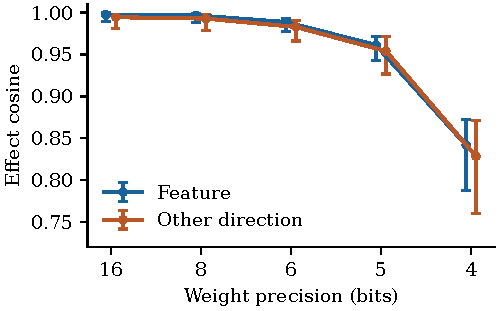
\includegraphics[width=\linewidth]{direction-control.pdf}
\caption{Median fingerprint similarity on the same 404 features and matched directions. Bars show interquartile ranges, not confidence intervals. The numerical drift is largely shared by alternative perturbations.}
\label{fig:directions}
\end{figure}

At INT5, about 31\% of features above the write-side reference fail activation survival. This is disagreement with an operational reference, not a semantic false-negative rate. Association status has descriptive AUROC 0.506 ($[0.469,0.543]$) for INT4 write-side similarity. The FP margin is much better at predicting association loss than functional change: on the same samples, INT6 AUROCs are 0.86 and 0.58, respectively. Thus, label stability and causal-effect stability should not be conflated.

\section{Graded Feature Scaling}
\subsection{Dose response across precision}
Study G varies $\alpha$ in Equation~\ref{eq:edit} for the same K64 groups. A separate 100-sentence FP pilot calibrates three down multipliers, 0.3536/0.1768/0.0884, to target increasing fractions of zero-ablation harm; up multipliers are their reciprocals, 2.8284/5.6569/11.3137. Fine increases of 1.1 and 1.2 are specified separately. The main evaluation uses 300 sentences, 27 languages, and three control draws.

In FP, median net harm increases from 0.0223 to 0.0902 to 0.1687 to 0.2624 as the group is suppressed more strongly and finally zeroed. The down-dose ordering holds in all 27 languages; 26 have a positive lower interval bound at the deepest nonzero down multiplier. Strong amplification also raises harm. The curves are similar from FP through INT5, with an INT4 increase (Figure~\ref{fig:gain}). The predefined strict precision-monotonicity rule is not met because a small intermediate decrease exceeds its tolerance. A post hoc relaxed tolerance is not substituted for that result.

\begin{figure}[t]
\centering
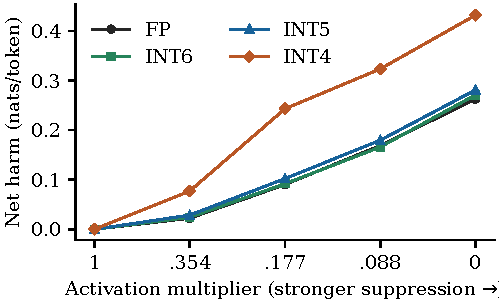
\includegraphics[width=\linewidth]{gain-down.pdf}
\caption{Median net harm under suppression, from the completed Study G curves. Net harm subtracts controls scaled by the same multiplier. The strongest precision change occurs at INT4.}
\label{fig:gain}
\end{figure}

\subsection{A small INT4 benefit and two checks}
The main sample suggests a small benefit from fine amplification at INT4 but is underpowered for that effect. The larger follow-up evaluates FP/INT6/INT5/INT4 on 562 reserve sentences per language, with five control draws and fixed primary multipliers 1.1 and 1.2. At INT4, 1.1 yields median net harm $-0.00135$ nats/token, with a 97.5\% interval $[-0.00197,-0.00032]$, and improves 20 of 27 languages. The 1.2 interval spans zero and its predefined rule is not met (Figure~\ref{fig:repair}). The matched controls do not show a clear corresponding decrease. The effect is approximately 0.05\% of loss, too small and narrowly evaluated to support a practical repair claim.

\begin{figure}[t]
\centering
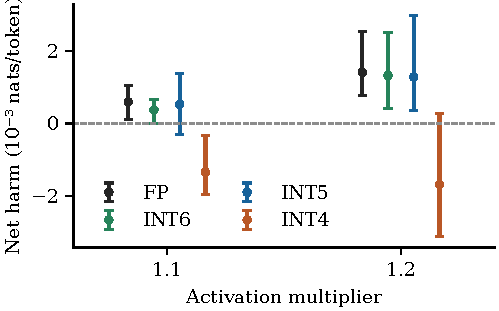
\includegraphics[width=\linewidth]{fine-gain.pdf}
\caption{Reserve-sentence follow-up: median net harm at small amplification ratios. Bars are the stored 97.5\% language-bootstrap intervals for the primary ratios. Negative values denote improvement relative to matched controls.}
\label{fig:repair}
\end{figure}

Two follow-ups test the interpretation. First, selecting each state's own top-64 language features changes membership substantially (INT4 Jaccard 0.49 with the FP selection), but the dose-response curves remain similar. State-defined groups are not more consequential than the FP reference: the median deepest-down net-harm difference at INT4 is $-0.0098$ nats/token. This supports robustness to group selection at this resolution, not identity of the underlying feature sets.

Second, the language-specific gain minimizing INT4 group harm is reproducible across sentence halves (reliability 0.917). Its rank correlation with inverse group-activation shrinkage is nevertheless $-0.170$ (one-sided permutation $p=0.804$). The smooth estimator agrees qualitatively. Therefore, a simple compensation explanation is not supported, even though the aggregate optimum and shrinkage can look compatible. We did not search many alternative predictors for a successful explanation.

\section{Discussion and Conclusion}
The original selective-destruction account is not established. Its primary contrasts were weak, its apparent threshold-dependent disadvantage changed after magnitude matching, and donor patches attributed little quantization loss to the selected language groups. Functional dependence on those groups persists on own-text prediction, but a frozen comprehension test does not establish the same dependence.

The strongest methodological lesson is to specify what a survival measurement preserves. A correlation cutoff describes activation agreement; a peak-language label depends on the margin to competing languages; a logit fingerprint describes a sampled intervention in a changing downstream model. None alone certifies an invariant language mechanism. The matched-direction control particularly limits the interpretation of functional drift: effects change at low precision, but they also change for perturbations that are not the feature's own direction.

For this course project, the outcome is a reproducible investigation that rejects parts of its motivating account and narrows others. We provide evidence of persistent group dependence, disagreement between survival views, and a small INT4 scaling benefit whose proposed compensation mechanism fails. These findings motivate better-calibrated compression audits; they do not establish a new quantization algorithm or broad multilingual capability recovery.

\label{main-content-end}
\section*{Limitations, Challenges, and Future Work}
One base model, layer, frozen SAE, and rounding scheme limit generalization. Dictionary fidelity can deteriorate after compression. Zero ablation can be off-distribution and does not establish unique necessity, sufficiency, or semantic identity. Imperfect matching and overlapping control draws constrain interpretation.

Most results are exploratory. Language tiers confound script, tokenization, training distribution, and competence. Bootstrap intervals condition on the selected sample; discrete peak labels introduce resampling bias. The numerical threshold is an operational choice, and averaged fingerprints can hide context dependence.

Challenges included replacing the initial pipeline, accelerator memory limits, hardware heterogeneity, and CUDA failures. Future work should replicate the measurements across models and quantizers, assess dictionary variability, use task interventions with calibrated headroom, and prospectively test predictors of useful gains. These extensions are not completed results.

\clearpage
\balance
\bibliography{references}

\clearpage
\nobalance
\appendix
\section{Language Panel and Reproduction}
\label{app:languages}
\begin{table}[htbp]
\centering
\begin{tabular}{lll}
\toprule
Tier & Language & FLORES code\\
\midrule
High & English & eng\_Latn\\
 & German & deu\_Latn\\
 & Spanish & spa\_Latn\\
 & French & fra\_Latn\\
 & Portuguese & por\_Latn\\
 & Russian & rus\_Cyrl\\
 & Chinese & zho\_Hans\\
 & Japanese & jpn\_Jpan\\
 & Korean & kor\_Hang\\
Mid & Hindi & hin\_Deva\\
 & Bengali & ben\_Beng\\
 & Tamil & tam\_Taml\\
 & Turkish & tur\_Latn\\
 & Vietnamese & vie\_Latn\\
 & Indonesian & ind\_Latn\\
 & Thai & tha\_Thai\\
 & Polish & pol\_Latn\\
 & Ukrainian & ukr\_Cyrl\\
Low & Kannada & kan\_Knda\\
 & Telugu & tel\_Telu\\
 & Yoruba & yor\_Latn\\
 & Sundanese & sun\_Latn\\
 & Amharic & amh\_Ethi\\
 & Igbo & ibo\_Latn\\
 & Hausa & hau\_Latn\\
 & Khmer & khm\_Khmr\\
 & Lao & lao\_Laoo\\
\bottomrule
\end{tabular}
\caption{The fixed 27-language roster. Tiers are descriptive project groupings informed by resource taxonomies, not a claim that languages have comparable training exposure within a tier.}
\end{table}

The repository is \url{https://github.com/TH4KUR/always-late}. The report's companion evidence map identifies the generated source tables and analysis files for each numerical block. The private artifact dataset is \url{https://huggingface.co/datasets/karma-skz/always-late-artifacts}; access or a subsequent public release is needed for its contents. Newer item-level functional files are recorded by location and checksum and are not all archived there yet.

The completed Phase 1 reproduction compared 89 output files against cached inputs and found all identical. The latest Study G and prompt-check reproduction compared 45 outputs with zero differences. These are regeneration checks of analyses, not independent repetitions of model inference. Evaluation freezes, sample identifiers, matching manifests, run metadata, and SHA-256 checksums identify the underlying runs. Standard-library and Torch test suites, mutation checks, sham gates, and restore-only identities provide additional implementation checks, not proof of the scientific interpretation.

\section{Hypotheses That Were Not Supported}
The historical selective-versus-control family did not reject after correction in the primary regime. The frozen Belebele S0 statement was not met, making S1--S5 undefined. The strict Study G precision-monotonicity rule failed. Its original repair rules were not met before the larger follow-up; the larger follow-up supported only the 1.1 primary multiplier. State-defined groups were not more consequential than FP-defined groups, and inverse activation shrinkage did not predict the optimal language-specific gain. These outcomes are preserved rather than omitted or converted into successful hypotheses by changing thresholds.

\end{document}
